\documentclass{beamer}
\usepackage{../tut-slides}
\usepackage{../mathoperatorsAuD}

\usepackage{csquotes}
\usepackage{cancel}

\usepackage{amsmath,amssymb}

\usepackage{tikz}
\usetikzlibrary{positioning,automata, matrix, trees}
\usetikzlibrary{calc,positioning,backgrounds,arrows.meta}
\usepackage{forest}


\usepackage{booktabs}
\usepackage{tabularx}
\usepackage{tabu}
\newcommand*\head{\rowfont{\bfseries}}
\newcommand*{\tw}{\rowfont{\ttfamily}}

\renewcommand{\tabularxcolumn}[1]{>{\hspace{0pt}}m{#1}}

\usepackage{listings}
\lstset{ 
	basicstyle=\footnotesize\ttfamily,        % the size of the fonts that are used for the code
	breakatwhitespace=false,         % sets if automatic breaks should only happen at whitespace
	breaklines=true,                 % sets automatic line breaking
	commentstyle=\itshape,    	     % comment style
	escapeinside={\%*}{*)},          % if you want to add LaTeX within your code
	extendedchars=true,              % lets you use non-ASCII characters; for 8-bits encodings only, does not work with UTF-8
	firstnumber=1,                % start line enumeration with line 1000
	frame=single,
	keywordstyle=\bfseries,       % keyword style
	morekeywords={}, 
	language=Prolog,                 % the language of the code
	numbers=left,                    % where to put the line-numbers; possible: (none, left, right)
	numbersep=5pt,                   % how far the line-numbers are from the code
	numberstyle=\tiny\color{cdgray!50}, % the style that is used for the line-numbers
	rulecolor=\color{cddarkblue}, 
	tabsize=2,	                   % sets default tabsize to 2 spaces
}

\lstdefinestyle{bg}{ 
	basicstyle=\footnotesize\ttfamily,        % the size of the fonts that are used for the code
	breakatwhitespace=false,         % sets if automatic breaks should only happen at whitespace
	breaklines=true,                 % sets automatic line breaking
	commentstyle=\itshape,    	     % comment style
	escapeinside={\%*}{\%*},          % if you want to add LaTeX within your code
	extendedchars=true,              % lets you use non-ASCII characters; for 8-bits encodings only, does not work with UTF-8
	firstnumber=1,                % start line enumeration with line 1000
	frame=L,
	backgroundcolor=\color{cdgray!15},
	%	keywordstyle=\bfseries,       % keyword style
	language=Haskell,                 % the language of the code
	numbers=left,                    % where to put the line-numbers; possible: (none, left, right)
	numbersep=8pt,                   % how far the line-numbers are from the code
	numberstyle=\tiny\color{cdgray!50}, % the style that is used for the line-numbers
	rulecolor=\color{cddarkblue}, 
	showstringspaces=false,
	tabsize=2,	                   % sets default tabsize to 2 spaces
}

\usepackage{textgreek}

\DeclareMathOperator{\GV}{GV}
\DeclareMathOperator{\FV}{FV}

\renewcommand{\emph}[1]{\textbf{#1}}
\newcommand{\coloremph}[1]{\textcolor{cdpurple}{#1}}
\newcommand{\col}[1]{\textcolor{cdpurple}{\boldsymbol{#1}}}
\newcommand{\coll}[1]{\textcolor{cddarkgreen}{\boldsymbol{#1}}}
\newcommand{\colll}[1]{\textcolor{cdorange}{\boldsymbol{#1}}}
%\newcommand{\step}[2][]{\ensuremath{\overset{{#1} (\text{#2})}{=}}}
%\newcommand*{\astep}[2][]{\ensuremath{\overset{{#1} (\text{#2})}&{=}}}

\newcommand{\num}[1]{\ensuremath{\langle #1 \rangle}}

\newcommand{\true}{\operatorname{true}}
\newcommand{\false}{\operatorname{false}}

\newcommand{\operator}[1]{\textbf{\textcolor{black}{#1}}}
\newcommand{\pred}[1]{\textrm{#1}}
\newcommand{\Fam}{\operator{Fam}}

\begin{document}	
	\title{Programmierung}
	\subtitle{Übung 8: Logikprogrammierung mit Prolog${}^-$}
	\author{Eric Kunze}
	\email{eric.kunze@tu-dresden.de}
	\city{TU Dresden}
	\date{30. Mai 2022}
%	\institute{Lehrstuhl für Grundlagen der Programmierung}
	\titlegraphic{
\includegraphics[width=2cm]{../TUD-white.pdf}}
	
	\maketitle
	

%%%%%%%%%%%%%%%%%%%%%%%%%%%%%%%%%%%%%%%%%%%%%%%%%%%%%%%%%%%%%%%%%%%%%%%%%%%%%

\begin{frame}[fragile] \frametitle{Inhalt}
	\begin{enumerate}
		\item Funktionale Programmierung
		\begin{enumerate}
			\item Einführung in Haskell: Listen
			\item Algebraische Datentypen
			\item Funktionen höherer Ordnung
			\item Typpolymorphie \& Unifikation
			\item Beweis von Programmeigenschaften
			\item \textlambda--Kalkül
		\end{enumerate}
		\item \textbf{Logikprogrammierung}
		\item Implementierung einer imperativen Programmiersprache
		\item Verifikation von Programmeigenschaften
		\item H${}_\text{0}$ -- ein einfacher Kern von Haskell
	\end{enumerate}
\end{frame}


\section{Logikprogrammierung und Prolog${}^-$}

\begin{frame} \frametitle{Ein einführendes Beispiel}
	\footnotesize
	Wir betrachten den folgenden Familienstammbaum:
	
	\begin{center}
		\begin{forest}
			for tree={
				child anchor=west,
				parent anchor=east,
				grow=east,
				draw,
				anchor=west,
				edge path={
					\noexpand\path[\forestoption{edge}]
					(.child anchor) -| +(-5pt,0) -- +(-5pt,0) |-
					(!u.parent anchor)\forestoption{edge label};
				},
			}
			[Albert
			[Berti
			[ Conrad 
			[ Erich ]
			[ Eva 
			[ Fritz ]
			]
			]
			[ Claudia ]
			]
			[Beate
			[ Dennis ]
			[ Daniel ]
			]
			]
		\end{forest}
		
		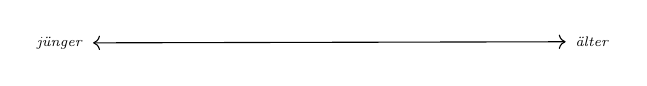
\begin{tikzpicture}[font=\tiny]
			\node[below left] (left) at (-3,0) {\textit{jünger}};
			\node[below right] (right) at (3,0) {\textit{älter}};
			\draw [<->] (left) -- (right);
		\end{tikzpicture}
	\end{center}
	
	Nun wollen wir die Verwandtschaftsbeziehungen abbilden. Dafür brauchen wir vor allem Geschlechter und Eltern-Kind-Beziehung(en).
	Dazu sei 
	\begin{align*}
		\Fam = \menge{albert, beate, berti, daniel, dennis, claudia, conrad, eva, erich, fritz}
	\end{align*}
	die Menge aller Familienmitglieder.
	
	\begin{tikzpicture}[remember picture, overlay]
		\node [
		font=\tiny\color{cdgray!80},  % Einstellungen für die Schrift
		inner xsep=0,       % Abstand des Textes von unten
		% maximale Textbreite = Papierhöhe - 2*Abstand des Textes von unten:
		%			text width={\dimexpr\paperheight-2\footskip\relax},
		align=center,
		%			minimum height=8mm,% Breite des Randstreifens
		anchor=south west,
		] at ($(current page.south west)+(+10mm,+2.5mm)$)
		{Wir betrachten hier den stark vereinfachten Fall und nehmen eine binäre Geschlechtsvorstellung an.};
	\end{tikzpicture}
\end{frame}

\begin{frame} \frametitle{Prädikatenlogik}
	\footnotesize
	\begin{itemize}
		\item \textit{Variablen}, z.B. $X$ $\leadsto$ kann verschiedene Werte annehmen
		\item \textit{Konstanten}, z.B. $albert$ $\leadsto$ fixer Wert
		\item \textit{Konstruktoren} (auch \enquote{Funktionen})
		\item \textit{Prädikate}, z.B. $male$ $\leadsto$ Wahrheit hängt von Argumenten ab 
		\begin{itemize} \footnotesize
			\item $male(albert) = \true$, aber $male(beate) = \false$
			\item $parent(claudia, berti) = \true$
		\end{itemize}
	\end{itemize}
	
	Prädikate kodieren Relationen passender Stelligkeit, d.h. beispielsweise
	\begin{align*}
		\operator{M} &= \menge{X \in \Fam : male(X) = \true} \\
		\operator{P} &= \menge{(X,Y) \in \Fam \times \Fam : parent(X,Y) = \true}
	\end{align*}

	\textbf{Problem:} Woher wissen wir, was wahr und was falsch ist?
\end{frame}

\begin{frame} \frametitle{Fakten \& Regeln}
	\footnotesize
	
	\textbf{Ziel:} wahre Aussagen beschreiben
	\bigskip
	
	\textbf{Fakten:} unabhängig von anderen Zuständen immer wahr
	\begin{itemize}
		\item Albert ist männlich: $male(albert) = \true$
		\item Claudia ist ein Elternteil von Berti: $parent(claudia, berti) = \true$
	\end{itemize}
	
	\textbf{Regeln:} Abhängigkeit von einem oder mehreren anderen Fakten
	\begin{itemize}
		\item Vater ist männliches Elternteil:
		$parent(X,Y) \land male(X) \implies father(X,Y)$ 
	\end{itemize}
\end{frame}

\begin{frame} \frametitle{Einführung in Prolog}
	\footnotesize
	\begin{itemize}
		\item Französisch: programmation en logique 
		\item hier: Teilsprache Prolog${}^-$
		\item \textbf{Interpreter:} \textit{swipl} \\ \url{https://www.swi-prolog.org/download/stable}
		\begin{itemize} \footnotesize
			\item Nutzung wie üblich im Terminal
			\item \texttt{swipl <filename>} startet die interaktive Session
		\end{itemize}
		\item \textbf{Online-Editor \& Interpreter:} \url{https://swish.swi-prolog.org/}
	\end{itemize}
	
	\bigskip \pause \hrule \medskip
	
	\begin{itemize}		
		\item Prolog-Programme bestehen aus \emph{Fakten} und \emph{Regeln}.
		\bigskip
		\item Statements werden mit \emph{\texttt{.}} abgeschlossen.
		\item Variablen beginnen mit Großbuchstaben.
		\bigskip
		\item \emph{UND}-Operator: \hspace{.25cm} \texttt{,}
		\item \emph{ODER}-Operator:\hspace{.2cm} \texttt{;}
	\end{itemize}
\end{frame}

\begin{frame}[fragile] \frametitle{Prolog: Fakten}
	\footnotesize
	
	\textbf{Ziel:} wahre Aussagen beschreiben
	
	
	\textbf{Fakten:} unabhängig von anderen Zuständen immer wahr
	
	\begin{itemize}
		\item männliche Familienmitglieder: \pause
		
		\begin{minipage}[t]{\dimexpr0.5\linewidth-\fboxrule-\fboxsep}
			\lstinputlisting[linerange={1-3}, frame=l, basicstyle=\ttfamily\scriptsize]{tut08-example-family.pl}
		\end{minipage}
		\begin{minipage}[t]{\dimexpr0.5\linewidth-\fboxrule-\fboxsep}
			\lstinputlisting[linerange={4-7}, frame=l, basicstyle=\ttfamily\scriptsize, firstnumber=4]{tut08-example-family.pl}
		\end{minipage} \pause
		%
		\item Elternbeziehungen: \pause
		
		\begin{minipage}[t]{\dimexpr0.5\linewidth-\fboxrule-\fboxsep}
			\lstinputlisting[linerange={9-14}, frame=l, basicstyle=\ttfamily\scriptsize, firstnumber= 9]{tut08-example-family.pl}
		\end{minipage}
		\begin{minipage}[t]{\dimexpr0.5\linewidth-\fboxrule-\fboxsep}
			\lstinputlisting[linerange={15-21}, frame=l, basicstyle=\ttfamily\scriptsize,firstnumber=15]{tut08-example-family.pl}
		\end{minipage} \pause
	\end{itemize}
\end{frame}

\begin{frame}[fragile] \frametitle{Prolog: Regeln}
	\footnotesize
	
	\textbf{Ziel:} wahre Aussagen beschreiben
	
	\textbf{Regeln:} Abhängigkeit von einem oder mehreren anderen Fakten
		
	\begin{itemize}
		\item Geschlecht weiblich: \pause
		\begin{lstlisting}[frame=l, basicstyle=\ttfamily\scriptsize,firstnumber=23]
female(X) :- not(male(X)).
		\end{lstlisting} \pause
		\item Prädikat $father$: \pause
		\begin{lstlisting}[frame=l, basicstyle=\ttfamily\scriptsize,firstnumber=25]
father(X,Y) :- parent(X,Y), male(X).
		\end{lstlisting} \pause
		\item Prädikat $ancestor$ --- Wir suchen eine Regel, um zu prüfen, ob $X$ ein Vorfahre von $Y$ ist.
		\pause
		Ein Elternteil ist immer auch ein Vorfahre; die Vorfahren eines Elternteils von $Y$ sind wiederum Vorfahren von $Y$.
		\pause
		\begin{lstlisting}[frame=l, basicstyle=\ttfamily\scriptsize,firstnumber=27]
ancestor(X,Y) :- parent(X,Y).
ancestor(X,Y) :- parent(Z,Y), ancestor(X,Z).
		\end{lstlisting}
	\end{itemize}
\end{frame}

\begin{frame} \frametitle{Arbeiten mit Swipl --- Anfragen}
	\footnotesize
	Nun möchten wir Programme auch ausführen. Aus Logik-Sicht ist die Ausführung eine Anfrage (\textit{query}): wir wollen wissen, ob ein Fakt gilt oder nicht (bzw. ob er gültig gemacht werden kann). Diesen Fakt nennen wir das Ziel (\textit{goal}).
	\begin{itemize}
		\item Ist Albert männlich?
		\item Anfrage: \texttt{?- male(albert).}
		\item Antwort: \texttt{true.}
	\end{itemize}

	\pause
	
	Im Allgemeinen gibt es kein I/O. Wir können das aber \enquote{simulieren}, indem wir Variablen nutzen. 
	\begin{itemize}
		\item Welche Personen sind männlich?
		\item Anfrage: \texttt{?- male(X).}
		\item Anzeigen mehrerer Lösungen in \texttt{swipl} durch \texttt{;}
	\end{itemize}

	Die Belegung einer solchen Variable lässt sich mittel SLD-Refutation unter Nutzung von Unifikationen ermitteln.
\end{frame}

\begin{frame} \frametitle{SLD-Refutationen}
	\footnotesize
	\textbf{Ziel:} zeige Gültigkeit einer Anfrage (eines Goals) $G = (\texttt{?- } L_1, \dots, L_n)$
	
	\textbf{SLD-Resolution:}
	\begin{itemize}
		\item wähle ein $L_i$ aus
		\item es gibt eine Regel $C = (M_0 \texttt{:- }M_1, \dots, M_m)$,\\
		wobei $C$ und $G$ keine gemeinsamen Variablen haben
		\item $\sigma$ sei der allgemeinste Unifikator von $L_i$ und $M_0$
	\end{itemize}
	\textbf{Dann:} ersetze $L_i$ durch $M_1, \dots, M_m$ unter Anwendung von $\sigma$ --- formal: 
	\begin{equation*}
		G' = \Big( \texttt{?- } \tilde{\sigma}(L_1), \dots \tilde{\sigma}(L_{i-1}) ,  \tilde{\sigma}(M_1), \dots, \tilde{\sigma}(M_m), \tilde{\sigma}(L_{i+1}), \dots, \tilde{\sigma}(L_n) \Big)
	\end{equation*}
	$G'$ heißt \textit{Resolvente} von $G$ und $C$ unter $\sigma$.
	
	\begin{itemize}
		\item\textbf{SLD-Ableitung} (derivation): Folge von SLD-Resolutionen
		\item \textbf{SLD-Refutation} (refutation): endliche Folge von SLD-Resolutionen mit dem leeren Goal \texttt{?-.} als Ende
	\end{itemize}
\end{frame}


%%%%%%%%%%%%%%%%%%%%%%%%%%%%%%%%%%%%%%%%%%%%%%%%%%%%%%%%%%%%%%%%%%%%%%%%%%%%%%%%


\section{Aufgabe 1}


\begin{frame}[fragile] \frametitle{Aufgabe 1}
	\centering
	
	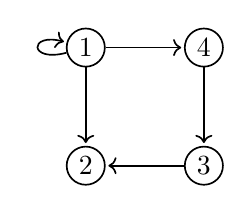
\begin{tikzpicture}[shorten >=1pt,node distance=1.5cm, semithick, on grid]
		\node[state, inner sep=2pt, minimum size=11pt]   (q_1)                {$1$};
		\node[state, inner sep=2pt, minimum size=11pt]   (q_2) [below=of q_1] {$2$};
		\node[state, inner sep=2pt, minimum size=11pt]   (q_3) [right=of q_2] {$3$};
		\node[state, inner sep=2pt, minimum size=11pt]   (q_4) [right=of q_1] {$4$};
		\path[->] (q_1) edge                node [above] {} (q_2)
		  			(q_3) edge                node [above] {} (q_2)
		  			(q_1) edge                node [above] {} (q_4)
		  			(q_4) edge                node [above] {} (q_3)
		(q_1) edge [loop left]    node [above] {} (q_1);
	\end{tikzpicture}
	\pause
	\begin{lstlisting}
edge(1,1).
edge(1,4).
edge(1,2).
edge(3,2).
edge(4,3).
	\end{lstlisting}
	\pause
	\begin{lstlisting}[firstnumber=7]
path(U, U).
path(U, W) :- edge(U, V), path(V, W).
	\end{lstlisting}
\end{frame}


\begin{frame} \frametitle{Aufgabe 1}
	\footnotesize
	
	\textit{ \tiny Hinweis: Die Zeilenangaben in den Refutationen können von denen in der Übung abweichen.}
	
	\vspace{-1em}
	
	\begin{minipage}{\dimexpr0.7\linewidth-\fboxrule-\fboxsep}
		\footnotesize
		\begin{alignat*}{2}
			&\texttt{?- path(4,X).} \\
			\texttt{\{X=4\}} \quad &\texttt{?- .} && \texttt{\% 7 } \\[12pt]
			%
			&\texttt{?- path(4,X).}  \\
			&\texttt{?- edge(4,W), path(W,X).} \quad && \texttt{\% 8} \\
			\texttt{\{W=3\}} \quad &\texttt{?- path(3,X).} && \texttt{\% 5} \\
			\texttt{\{X=3\}} \quad &\texttt{?- .} && \texttt{\% 6}\\[12pt]
			%
			&\texttt{?- path(4,X).}  \\
			&\texttt{?- edge(4,W), path(W,X).} \quad && \texttt{\% 8} \\
			\texttt{\{W=3\}} \quad &\texttt{?- path(3,X).} && \texttt{\% 5} \\
			&\texttt{?- edge(3,U), path(U,X).} &&\texttt{\% 8} \\
			\texttt{\{U=2\}} \quad &\texttt{?- path(2,X).} &&\texttt{\% 4} \\
			\texttt{\{X=2\}} \quad &\texttt{?- .} &&\texttt{\% 7} \\
		\end{alignat*}
	\end{minipage}
	\begin{minipage}{\dimexpr0.3\linewidth-\fboxrule-\fboxsep}
		\vfill \centering
		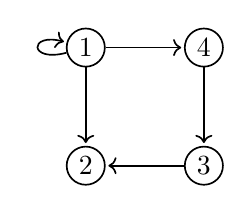
\begin{tikzpicture}[shorten >=1pt,node distance=1.5cm, semithick, on grid]
			\node[state, inner sep=2pt, minimum size=11pt]   (q_1)                {$1$};
			\node[state, inner sep=2pt, minimum size=11pt]   (q_2) [below=of q_1] {$2$};
			\node[state, inner sep=2pt, minimum size=11pt]   (q_3) [right=of q_2] {$3$};
			\node[state, inner sep=2pt, minimum size=11pt]   (q_4) [right=of q_1] {$4$};
			\path[->] (q_1) edge                node [above] {} (q_2)
			(q_3) edge                node [above] {} (q_2)
			(q_1) edge                node [above] {} (q_4)
			(q_4) edge                node [above] {} (q_3)
			(q_1) edge [loop left]    node [above] {} (q_1);
		\end{tikzpicture}
		\vfill
	\end{minipage}
\end{frame}


%%%%%%%%%%%%%%%%%%%%%%%%%%%%%%%%%%%%%%%%%%%%%%%%%%%%%%%%%%%%%%%%%%%%%%%%%%%%%%%%


\section{Aufgabe 2}

\begin{frame}[fragile] \frametitle{Arithmetik in Prolog: natürliche Zahlen}
	\footnotesize
	\textbf{natürliche Zahlen:} Unärkodierung mit Konstruktor \texttt{s}, 
	\begin{equation*}
		\mathtt{
		\num{n} \defeq \underbrace{s( \cdots s}_{n \text{ mal}} (0))
		}
	\end{equation*}
	und einstelliges Prädikat \texttt{nat}, das über klassische Rekursion definiert ist:
	\begin{lstlisting}[frame=l]
nat(0).
nat(s(X)) :- nat(X).
	\end{lstlisting}

	\pause \scriptsize
	
	\textbf{Anmerkung 1:} Prolog weiß dabei nicht, dass es sich um Zahlen handelt. Vielmehr sind alle Zeichen nur Symbole; die Zahl \texttt{0} wird zum Beispiel als Konstante im Sinne der Prädikatenlogik angesehen.
	\pause
	
	\textbf{Anmerkung 2:} Durch die Unärkodierung müssen wir bei rekursiven Funktionen ein wenig umdenken. Die Zahl $\num{n}$ lässt sich in einer Rekursion nicht auf $\num{n-1}$ reduzieren. Stattdessen fügen wir vorher ein \texttt{s} ein, um es anschließend wieder zu entfernen, d.h. $\num{n+1} \leadsto \num{n}$.
	\begin{itemize}
		\item Haskell-Rekursion: $n \leadsto n-1$
		\item Prolog-Rekursion: $n+1 \leadsto n$
	\end{itemize}

\end{frame}

\begin{frame}[fragile] \frametitle{Arithmetik in Prolog: Funktionen}
	\footnotesize
	
	Funktionen müssen als Relationen dargestellt werden, d.h. 
	\begin{align*}
		\text{statt } \qquad
		\begin{aligned}
			f : \N \to \N \\
			f(x) = y
		\end{aligned}
		\quad
		\text{ kodieren wir }
		\quad \operator{F} = \menge{(x,y) \in \N \times \N : f(x) = y }
	\end{align*}
	\pause
	
	\textbf{Beispiel:} Summe zweier natürlicher Zahlen
	
	rekursive Idee:
	\begin{align*}
		0 + y = y \enskip &\impliedby \enskip y \in \N \tag{Basisfall} \\
		(x+1) + y = s+1 \enskip &\impliedby \enskip x + y = s \tag{Rekursionsfall}
	\end{align*}
	\pause
	
	\begin{minipage}[t]{\dimexpr0.5\linewidth-\fboxrule-\fboxsep}
		Haskell:
		\begin{lstlisting}[basicstyle=\ttfamily\scriptsize, frame=l]
sum :: Int -> Int -> Int
sum 0 y = y
sum x y = 1 + sum (x-1)  y
		\end{lstlisting}
	\end{minipage}
	\begin{minipage}[t]{\dimexpr0.5\linewidth-\fboxrule-\fboxsep}
		Prolog:
		\begin{lstlisting}[basicstyle=\ttfamily\scriptsize, frame=l]
			
sum(0, Y, Y) :- nat(Y).
sum(s(X), Y, s(S)) 
             :- sum(X, Y, S).
		\end{lstlisting}
	\end{minipage}
\end{frame}

\begin{frame}[fragile] \frametitle{Aufgabe 2 -- Teil (a)}
	\footnotesize
	\begin{lstlisting}
nat(0).
nat(s(X)) :- nat(X).

sum(0, Y, Y) :- nat(Y).
sum(s(X), Y, s(S)) :- sum(X, Y, S).
	\end{lstlisting}
	
	\textbf{Gesucht:} Prädikat \texttt{even}, dass alle natürlichen Zahlen enthält
	
	\pause
	
	\begin{lstlisting}[firstnumber=7]
even(0).
even(s(s(N))) :- even(N).
	\end{lstlisting}
\end{frame}

\begin{frame}[fragile] \frametitle{Aufgabe 2 -- Teil (b)}
	\footnotesize
	\begin{lstlisting}
nat(0).
nat(s(X)) :- nat(X).

sum(0, Y, Y) :- nat(Y).
sum(s(X), Y, s(S)) :- sum(X, Y, S).

even(0).
even(s(s(N))) :- even(N).
	\end{lstlisting}
	
	\textbf{Gesucht:} Relation \texttt{div2} mit $(\num{\texttt{n}} , \num{\lfloor \frac{\texttt{n}}{\texttt{2}} \rfloor})$
	
	\pause
	
	\begin{lstlisting}[firstnumber=10]
div2(0, 0).
div2(s(0), 0).
div2(s(s(N)), s(M)) :- div2(N, M).
	\end{lstlisting}
\end{frame}

\begin{frame}[fragile] \frametitle{Aufgabe 2 --Teil (c)}
	\begin{lstlisting}[firstnumber=10]
div2(0, 0).
div2(s(0), 0).
div2(s(s(N)), s(M)) :- div2(N, M).
	\end{lstlisting}

	\textbf{gesucht:} SLD-Refutation für \texttt{?- div2(<3>, <1>).}
	
	\begin{alignat*}{2}
		&\texttt{?- div2(<3>, <1>).} \\
		&\texttt{?- div2(<1>, 0).} \qquad && \texttt{\% 12 } \\
		&\texttt{?- .} && \texttt{\% 11 }
	\end{alignat*}
\end{frame}

\begin{frame}[fragile] \frametitle{Aufgabe 2 -- Teil (d) \hfill \textit{Zusatz}}
	\footnotesize
	\begin{lstlisting}
nat(0).
nat(s(X)) :- nat(X).

sum(0, Y, Y) :- nat(Y).
sum(s(X), Y, s(S)) :- sum(X, Y, S).
	\end{lstlisting}
	
	\textbf{Gesucht:} Relation \texttt{div} mit $(\num{\texttt{n}} , \num{\texttt{m}} , \num{\lfloor \frac{\texttt{n}}{\texttt{m}} \rfloor})$
	
	\pause
	
	\begin{lstlisting}[firstnumber=14]
lt(0, s(M)) :- nat(M).
lt(s(N), s(M)) :- lt(N, M).
	\end{lstlisting}
	
	\pause
	
	\begin{lstlisting}[firstnumber=17]
div(0, M, 0) :- lt(0, M).
div(N, M, 0) :- lt(N, M).
div(N, M, s(Q)) :- lt(0, M), sum(M, V, N), 
                   div(V, M, Q).
	\end{lstlisting}
\end{frame}

\begin{frame} \frametitle{Aufgabe 2 -- Teil (e) \hfill \textit{Zusatz}}
	\scriptsize
	\begin{alignat*}{2}
		&\texttt{?- div(\num{3}, \num{2}, \num{1})} \\
		&\texttt{?- lt(\num{0}, \num{2}) , sum(\num{2}, V1, \num{3}) , div(V1, \num{2}, \num{0})} \qquad && \texttt{\% 19 } \\
		&\texttt{?- nat(\num{1}) , sum(\num{2}, V1, \num{3}) , div(V1, \num{2}, \num{0})}  && \texttt{\% 14} \\
		&\texttt{?- nat(\num{0}) , sum(\num{2}, V1, \num{3}) , div(V1, \num{2}, \num{0})} && \texttt{\% 2} \\
		&\texttt{?- sum(\num{2}, V1, \num{3}) , div(V1, \num{2}, \num{0}).} && \texttt{\% 1} \\
		&\texttt{?-* sum(\num{0}, V1, \num{1}) , div(V1, \num{2}, \num{0}).} && \texttt{\% 4} \\
		\texttt{\{V1=\num{1}\}} \quad &\texttt{?- nat(\num{1}) , div(\num{1}, \num{2}, \num{0}).} && \texttt{\% 3} \\
		&\texttt{?- nat(\num{0}) , div(\num{1}, \num{2}, \num{0}).} \quad && \texttt{\% 2} \\
		&\texttt{?- div(\num{1}, \num{2}, \num{0}).} && \texttt{\% 1} \\
		&\texttt{?- lt(\num{1}, \num{2}).} &&\texttt{\% 18} \\
		&\texttt{?- lt(\num{0}, \num{1}).} &&\texttt{\% 15} \\
		&\texttt{?- nat(\num{0}).} &&\texttt{\% 14} \\
		&\texttt{?- .} &&\texttt{\% 1} \\
	\end{alignat*}
\end{frame}

\end{document}

